\chapter{一元函数微分学}

\section{导数与微分}

\subsection{导数的概念与计算}

导数的概念高中已经学过, 这里只是快速回顾(和严格化): 

\begin{definition}{导数}
	设$f:E \to \R$, $f$在$x_0$附近有定义. 称$f$在$x_0$处\textit{可导}(derivable), 如果下列极限存在(且有限): 
	$$\lim_{\Delta x \to 0} \frac{f(x_0+\Delta x) - f(x_0)}{\Delta x}, $$
	并记$f$在$x_0$的\textit{导数}(derivative)为该极限值. 
\end{definition}
\begin{remark}
	若$f$在$x_0$处可导, 显然$f$在$x_0$处连续. (反之则不一定! 如$f(x)=|x|$在$x=0$处连续但不可导)
\end{remark}
\begin{remark}
	$f$在$x_0$处的导数有以下主流记号: $$f'(x_0),\quad \frac{\dif }{\dif x} f(x) \big|_{x=x_0},\quad \dot{f}(x_0). $$
	第一种比较常见; 第二种将导数和微分联系起来(但现在我们暂且将其看做算子), 并提示我们考虑$f$的逐点导数; 第三种在物理学中常见. 
\end{remark}
\begin{remark}
	若$f$在$E$上逐点可导, 则称$f':E \to \R ,x \to f'(x)$为其导(函)数. 若$f'$连续, 则称$f$($1$-阶)连续可导, 并记所有这样的函数组成集合$C^1(E)$. 
\end{remark}
\begin{remark}
	若$f'$仍然在$E$上可导, 我们可以求出$f$的二阶导数$f''$, 以此类推. 一般地, 记$f$的$n$阶导数为$f^{(n)}$或$\frac{\dif ^n f}{\dif x^n}$. 另外, 若$f^{(n)}$是连续的, 则称$f$是$n$-阶连续可导的, 记所有这样的函数组成集合$C^{n}(E)$. 
\end{remark}
\begin{remark}
	当然可以定义所谓单侧导数, 并注意到$f$在$x_0$处可导当且仅当左导数$f'_-(x_0)$等于右导数$f'_+(x_0)$. 
\end{remark}
\begin{remark}
	当然可以定义导数为无穷的情况, 但我们不认为这是可导. 
\end{remark}

注意到, 若$f$在$x_0$处可导, 则$f$在局部可以写成以下形式: $$f(x_0+\Delta x) = f(x_0) + f'(x_0) \Delta x + o(\Delta x),\quad \Delta x \to 0. $$
该式子实际上就引入了微分的概念(见下一小节). 

\begin{proposition}{导数的四则运算}
	设$f,g$在$x$处可导. 则: 
	\begin{itemize}
		\item $f \pm g$在$x$处可导, 且$(f \pm g)'(x) = f'(x) \pm g'(x)$. 
		\item $f \cdot g$在$x$处可导, 且$(f\cdot g)'(x)=f'(x)g(x)+f(x)g'(x)$.
		\item (若$g \not\equiv 0$)$\frac{f}{g}$在$x$处可导, 且$\displaystyle \big( \frac{f}{g} \big)'(x) = \frac{f'(x)g(x)-f(x)g'(x)}{(g(x))^2}$. 
	\end{itemize}
\end{proposition}
\begin{proof}
	读者应当在中学就完成了这些公式的证明. 
\end{proof}

\begin{proposition}{Leibniz公式}
	设$f,g$在$x$处存在$n$次导数, 则
	\begin{center}
		$\displaystyle (f \cdot g)^{(n)}(x) = \sum_{k=0}^{n} \binom{n}{k} f^{(k)}(x)g^{(n-k)}(x)$. 
	\end{center}
\end{proposition}
\begin{proof}
	用归纳法和基本的组合数知识可以证明. 
\end{proof}

\begin{theorem}{复合函数的导数(链式法则)}
	设$f$在$x_0$处可导, $g$在$f(x_0)$处可导, 则$g\circ f$在$x_0$处可导, 且
	\begin{center}
		$(g\circ f)'(x_0)=g'(f(x_0))f'(x_0)$. 
	\end{center}
\end{theorem}
\begin{remark}
	复合函数的$n$次导数也有公式, 就是所谓Faà di Bruno公式. 
\end{remark}
\begin{proof}
	由之前的公式, 可知$$f(x_0+h)=f(x_0)+f'(x_0)h+o(h),\qquad g(f(x_0)+\ell )=g(f(x_0))+g'(f(x_0))\ell +o(\ell ).$$
	于是
	\begin{align*}
		\frac{g(f(x_0+h))-g(f(x_0))}{h} &= \frac{g( f(x_0)+f'(x_0)h+o(h) ) - g(f(x_0))}{h} \\
		&= \frac{g'(f(x_0)) \cdot (f'(x_0)h+o(h)) + o(f'(x_0)h+o(h))}{h} \\
		&= g'(f(x_0)) \cdot \left(f'(x_0) + \frac{o(h)}{h} \right) + o\left( f'(x_0)+\frac{o(h)}{h} \right) \\
		&\to g'(f(x_0))f'(x_0),\quad h \to 0. 
	\end{align*}
	其中, 我们令$\ell = f'(x_0)h+o(h)$, 显然当$h\to 0$时$\ell \to 0$, 因此上方的代换是合理的. 
\end{proof}
\begin{remark}
	如果直接用导数的定义式计算, 可能会出现$f(x)-f(x_0)$出现在分母上且为$0$的情况. 
\end{remark}

链式法则这个名字源自于上方定理的Leibniz记号表示: $$\frac{\dif z}{\dif x} = \frac{\dif z}{\dif y} \cdot \frac{\dif y}{\dif x}. $$
其中$z=g \circ f, y=f$. 我们不应将这个式子视作是简单的消元. 

\begin{theorem}{反函数的导数} \label{thm:fjhjuudedcuu}
	设$f$在区间$I$上连续且可逆. 若$f$在$x_0$处可导且$f'(x_0) \neq 0$, 则$f^{-1}$在$y_0=f(x_0)$处可导, 且有$$(f^{-1})'(y_0)=\frac{1}{f'(f^{-1}(y_0))}. $$
\end{theorem}
\begin{remark}
	一个小提醒: 若函数在一点连续, 其反函数不一定在该点对应的函数值处连续. (构造反例并不简单)
\end{remark}
\begin{proof}
	由$f$连续且可逆, 不妨设$f$单调递增, 那么$f^{-1}$单调递增且连续. 设$f(x_0)=y_0$, 则对于$y_0$的某个邻域$N_{\varepsilon}(y_0)$, 若$f^{-1}N_{\varepsilon}(y_0) = (x_0-\delta _1,x_0+\delta _2)$, 则当$y$从左至右遍历$N_{\varepsilon}(y_0)$时, $f^{-1}(y)$恰好从左至右遍历$(x_0-\delta _1,x_0+\delta _2)$. 特别地, $y \to y_0$等价于$x \to x_0$. 于是$$\lim_{y \to y_0} \frac{f^{-1}(y)-f^{-1}(y_0)}{y-y_0} = \lim_{y \to y_0} \left( \frac{f(x)-f(x_0)}{x-x_0} \right)^{-1} = \left( \lim_{x \to x_0}  \frac{f(x)-f(x_0)}{x-x_0} \right)^{-1} = \frac{1}{f'(x_0)}. $$
	其中, 第二个等号用到了上方“方向一致的一一对应”的想法. 
\end{proof}

现在来计算一些函数的导数: 

\begin{example}
	求$f(x)=e^x$的导数. 
\end{example}
\begin{solution}
	前面证明过, $\lim_{x \to 0} \frac{e^x-1}{x} = 1$. 于是$$\lim_{\Delta x \to 0} \frac{e^{x_0+\Delta x} - e^{x_0}}{\Delta x} = e^{x_0} \lim_{\Delta x \to 0} \frac{e^{\Delta x}-1}{\Delta x} = e^{x_0}. $$
	即$f'(x)=e^x$. 
\end{solution}

\begin{example}
	求$f(x) = \ln x$的导数. 
\end{example}
\begin{solution}
	一方面, 由反函数导数定理可以直接得到$f'(x)=\frac{1}{x}$. 另一方面, 亦可以注意到$$\lim_{\Delta x \to 0} \frac{\ln (x_0+\Delta x) - \ln x_0}{\Delta x} = \lim_{\Delta x \to 0} \frac{\ln \left( (1+\frac{\Delta x}{x_0})^{\frac{x_0}{\Delta x}} \right)}{x_0} = \frac{\ln \left(\lim_{\Delta x \to 0}  (1+\frac{\Delta x}{x_0})^{\frac{x_0}{\Delta x}} \right)}{x_0} = \frac{1}{x_0}. $$
\end{solution}

\begin{example}
	求$f(x)= \sin x$的导数. 
\end{example}
\begin{solution}
	注意到$$\lim_{\Delta x \to 0} \frac{\sin (x_0+\Delta x) - \sin x_0}{\Delta x} = \lim_{\Delta x \to 0} \frac{2\cos (x_0+\frac{\Delta x}{2}) \sin \frac{\Delta x}{2}}{\Delta x} = \cos \left( \lim_{\Delta x \to 0}\left( x_0+\frac{\Delta x}{2} \right) \right) \cdot \lim_{\Delta x \to 0} \frac{\sin \frac{\Delta x}{2}}{\frac{\Delta x}{2}} = \cos x_0. $$
\end{solution}

\begin{example}
	定义\textit{双曲正弦函数}$\sinh x:= \frac{1}{2}(e^x-e^{-x})$, \textit{双曲余弦函数}$\cosh x := \frac{1}{2}(e^x+e^{-x})$. 不难验证$\sinh$是单增的奇函数, $\cosh$是恒正的偶函数. 另外双曲函数具有和三角函数类似的性质, 如$\cosh ^2x - \sinh ^2x = 1$. 
	
	计算$\sinh x$和$\arsinh y$的导数. 
\end{example}
\begin{solution}
	易见$(\sinh x)'=\frac{1}{2}(e^x+e^{-x})=\cosh x$. 另外, 计算可得$\arsinh y = \ln (y+\sqrt{1+y^2})$. 于是$$(\arsinh y)' = \frac{1}{y+\sqrt{1+y^2}} \cdot \left( 1+\frac{y}{\sqrt{1+y^2}} \right) = \frac{1}{\sqrt{1+y^2}}. $$
\end{solution}
\begin{remark}
	我们注意到利用$e^x$的表示形式很容易求出$\arsinh$的导数. 类似地, $\sin x = \frac{1}{2}(e^{\ic x} - e^{-\ic x})$. 这启发我们研究复数域$\C$(或者说$\R ^2$)上函数的导数. 
\end{remark}

现在给出一张常见函数的导数表: 

\begin{figure}[H]
	\centering
	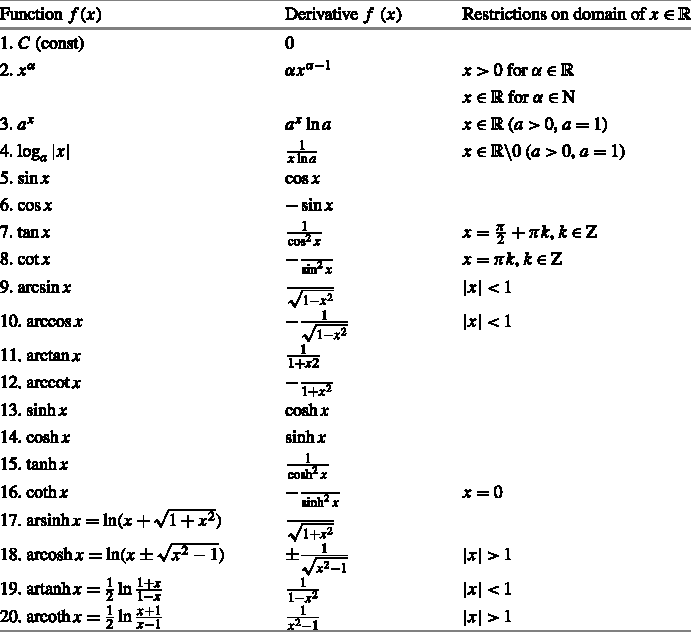
\includegraphics[width=13.5cm]{attachment/常见函数的导数.pdf}
	\caption{常见函数的导数表, 图源Zorich Table 5.1}
\end{figure}

\subsection{微分的概念}

上一节我们提到了这样一个公式: $$\Delta f(x) = f(x_0+\Delta x) - f(x_0) = f'(x_0) \Delta x + o(\Delta x),\quad \Delta x \to 0. $$
也就是说, 我们找到了一个线性函数$f'(x_0)\Delta x$来近似$\Delta f(x)$, 并且误差是关于$\Delta x$的无穷小量. 这样就产生了一个问题: 系数是$f'(x_0)$的线性函数的近似程度是否是最佳的? 我们会在后面给出解答. 

\begin{definition}{微分}
	设$f$在$x_0$附近有定义, 若存在$\lambda \in \R$使得$$f(x_0+\Delta x)-f(x_0) = \lambda \Delta x+o(\Delta x),\quad \Delta x \to 0,$$
	则称$f$在$x_0$处\textit{可微}(differentiable), 线性函数$\lambda \Delta x$为$f$在$x_0$处的\textit{微分}(differential), 记作$\dif f(x_0)$. 
\end{definition}

由上方的公式可知, 若$f$在$x_0$处可导, 则一定可微, 且系数$\lambda = f'(x_0)$. 反过来, 若$f$在$x_0$处可微, 在定义式的两边除以$\Delta x$并令$\Delta x \to 0$, 即得$f'(x_0) = \lambda$, 特别地$f$在$x_0$处可导. 

我们知道对于线性函数$f(x)=x$, 其微分恰好为$\Delta x$, 因此可以用记号$\dif x$代替$\Delta x$. 于是就有

\begin{proposition}{一元函数导数与微分的关系}
	一元函数$f$在$x_0$处可微当且仅当$f$在$x_0$处可导, 且
	\begin{center}
		$\dif f(x_0) = f'(x_0) \dif x. $
	\end{center}
\end{proposition}

该命题说明了记号$f'(x_0) = \frac{\dif f}{\dif x} \big|_{x=x_0}$的实际意义. 另外, 结合链式法则, 我们可以得到$$\dif g(f(x)) = g'(f(x)) f'(x)\dif x = g'(f(x)) \dif f(x). $$
该公式会在不定积分一节经常使用. 

从几何的观点来看, 在寻找一条曲线的切线时, 我们希望将切线定义为割线的极限位置, 而微分看起来就是这条切线(的某条平行线). 用形式化的语言写出来就是下方的定理: 

\begin{theorem}{微分最佳逼近定理}
	设$f$在$x_0$处可微, $\ell$是$f$在$x_0$处的\textit{切线}(tangent line), 定义为$\ell (x) = f(x_0)+f'(x_0)(x-x_0). $ \\
	则对于任意不等于$\ell (x)$的一次多项式$L(x)$都存在$\delta >0$, 使得对任意$x \in \mathring{N}_{\delta}(x_0)$都有
		$$|f(x)-\ell (x)| < |f(x)-L(x)|.$$
\end{theorem}
\begin{proof}
	当$L(x_0) \neq f(x_0)$时, 注意到$$\lim_{x \to x_0} |f(x) - L(x)| = |f(x_0)-L(x_0)|>0=\lim_{x\to x_0}|f(x)-\ell (x)|.$$
	由极限保序性知原命题成立. 
	
	当$L(x_0) = f(x_0)$时, 记$L(x)=f(x_0)+k(x-x_0)$, 那么$$\frac{|f(x)-\ell (x)|}{|f(x)-L(x)|} = \frac{o(x-x_0)}{(f'(x_0)-k)(x-x_0)+o(x-x_0)} \to 0,\quad x \to x_0. $$
	立得原命题成立. 
\end{proof}

\begin{figure}[H]
	\centering
	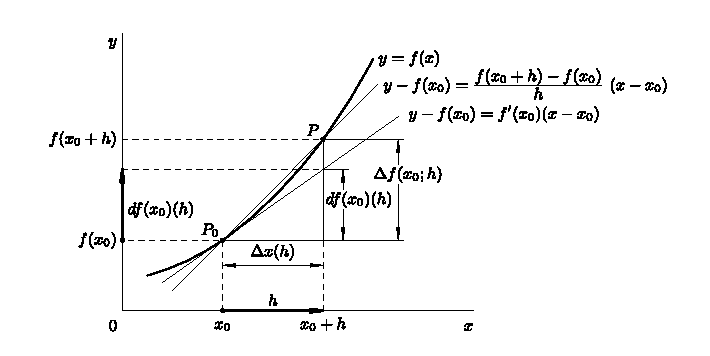
\includegraphics[width=12cm]{./attachment/differential_of_a_function.pdf}
	\caption{函数的割线, 切线, 微分等概念的示意图, 图源Zorich Fig. 5.3}
\end{figure}

利用微分形式, 可以较为方便地做计算. 

\begin{example}
	有些时候我们会遇到一些不便于写成显式表达式的函数, 例如椭圆方程$\displaystyle \frac{x^2}{a^2}+\frac{y^2}{b^2}=1$. 这时一般有两种表达方式: 隐式方程(即上式)或参数方程$\begin{cases}
	x=a\cos \theta \\ y=b\sin \theta
\end{cases},\theta \in [0,2\pi )$. 那么可以按如下方式求导: 
$$1)\quad 0 = \frac{\dif}{\dif x} 1 = \frac{\dif}{\dif x} \frac{x^2}{a^2} + \frac{\dif}{\dif x} \frac{y^2}{b^2} = \frac{2x}{a^2} + \frac{1}{b^2} \cdot \frac{\dif y^2}{\dif y} \cdot \frac{\dif y}{\dif x} = \frac{2x}{a^2} + \frac{2y}{b^2} \cdot y'\qquad \Leftrightarrow \qquad y' = -\frac{b^2x}{a^2y}. $$
并且注意到这样求出来的导数并不需要将椭圆拆成两半(以此保证函数良定义), 只需要将对应的横纵坐标代入. 
$$2)\quad y' = \frac{\dif y}{\dif x} = \frac{\dif y}{\dif \theta} \cdot \left( \frac{\dif x}{\dif \theta} \right)^{-1} = -\frac{b}{a} \cdot \frac{1}{\tan \theta} = -\frac{b^2x}{a^2y}. $$
当然最后一步代换不是必要的(因为一般写参数方程就是为了统一自变量). 
\end{example}

\begin{example}
	设$f$在$x$处存在$2$阶导数. 那么
	\begin{center}
		$\dif ^2 f(x) := \dif (\dif (f(x))) = \dif (f'(x) \dif x) = (f'(x) \dif x)' \dif x = f''(x) (\dif x)^2 =: f''(x) \dif x^2. $
	\end{center}
	注意在第4个等号处, $\dif x=\Delta x$是关于$x$的常数, 因此可以直接提出来. 这说明了高阶导数记号的意义. 
\end{example}



\newpage
\section{微分学的中值定理}

\subsection{函数的导数与其局部性质}

为了得到后面的重要定理, 我们先来研究导数所引出的函数局部性质: 

\begin{lemma}{}
	设开区间$I \subseteq \R$, $f:I \to \R$在$x_0$处可导且$f'(x_0)>0$. 那么存在$x_0$的邻域$N_{\delta}(x_0)$使得$f(x)-f(x_0)$在$x_0+\delta>x>x_0$时恒正, 在$x_0-\delta<x<x_0$时恒负. 
\end{lemma}
\begin{proof}
	易知存在$\delta$使得对任意$x\in N_{\delta}(x_0)$, $$\left| \frac{f(x)-f(x_0)}{x-x_0}-f'(x_0) \right| < \frac{1}{2}f'(x_0) \quad \Rightarrow \quad \frac{f(x)-f(x_0)}{x-x_0} > \frac{1}{2}f'(x_0) >0.$$
	即$f(x)-f(x_0)$与$x-x_0$同号. 
\end{proof}

\begin{proposition}{}
	设开区间$I\subseteq \R$, $f:I \to \R$在$I$上可导且对任意$x \in I$, $f'(x)>0$, 则$f$在$I$上严格单调递增. 
\end{proposition}
\begin{remark}
	该命题的不足之处在于: 若$f'(x) \geq 0$, 我们并不能说明$f$是单调不减函数. 这一结论将利用中值定理证明. 
\end{remark}

在下方的定理中, 局部极大(极小)值的定义为: 若存在邻域$N_{\delta}(x_0)$使得$f(x_0)$是$f$在$N_{\delta}(x_0)$上的最大(小)值, 则称$f(x_0)$为局部极大(极小)值. 

\begin{lemma}{Fermat引理}
	设$f:E \to \R$在$x_0$处可导, 则$f$在$x_0$处取得局部极值的必要条件是$f'(x_0)=0$. 
\end{lemma}
\begin{proof}
	设若不然, 不妨$f'(x_0)>0$, 则在$x_0$的某个邻域中对$x>x_0$总有$f(x)>f(x_0)$, 故$f(x_0)$不是局部极大值, 同理也不是局部极小值. 
\end{proof}

一般地, 称使得$f'(x_0)=0$的点$x_0$为$f$的\textit{驻点}(stationary point). 后面会看到, 通过计算$f''(x_0)$可以判断一个驻点$x_0$是否是极值点以及$f(x_0)$是极大值还是极小值. 

\subsection{Lagrange中值定理}

回顾\textit{无穷小增量公式}: $$f(x+h)-f(x)=f'(x)h+o(h),\quad h \to 0.$$
我们可以发现, 当$h \to 0$时, 上述公式实际上在用某点处的导数和定义域长度$h$的乘积描述$f$在初末位置取值的差. 那么能否将$h \to 0$的情况推广? 即让$f:[a,b] \to \R$, 是否存在$\xi \in [a,b]$使得$f(b)-f(a)=f'(\xi) (b-a)$? 我们从一个必要的情况出发考虑, 并将其作为引理. 

\begin{theorem}{Rolle中值定理}
	设$f$在$[a,b]$上连续, 在$(a,b)$上可导. 若$f(a)=f(b)$, 则存在$\xi \in (a,b)$使得$f'(\xi )=0$. 
\end{theorem}
\begin{proof}
	由$f$在$[a,b]$上连续可知$f$可取得最大值$M$和最小值$m$. 若$M=m$则$f'(x) \equiv 0$; 若$M>m$, 不妨$M>f(a)=f(b)$, 则存在$\xi$使得$f(\xi)=M$即$f'(\xi) = 0$. 
\end{proof}

\begin{theorem}{Lagrange中值定理}
	设$f$在$[a,b]$上连续, 在$(a,b)$上可导. 则存在$\xi \in (a,b)$使得$f'(\xi) = \dfrac{f(b)-f(a)}{b-a}$. 
\end{theorem}
\begin{remark}
	等价且好用的说法是: 存在$\theta \in (0,1)$使得$f'(a+\theta h)=\frac{f(a+h)-f(a)}{h}$, 其中$h=b-a$. 
\end{remark}
\begin{proof}
	构造函数$F(x)=f(x)-\frac{f(b)-f(a)}{b-a}(x-a)$, 则$F(a)=F(b)=f(a)$, 所以存在$\xi \in (a,b)$使得$F'(\xi)=0$, 也就是$f'(\xi) = \frac{f(b)-f(a)}{b-a}$. 
\end{proof}

\begin{figure}[H]
	\centering
	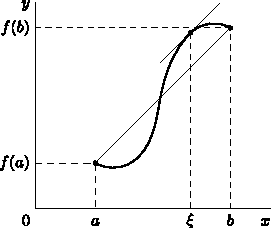
\includegraphics[width=6cm]{./attachment/Lagrange中值定理.pdf}
	\caption{Lagrange中值定理示意图, 图源Zorich Fig. 5.9}
\end{figure}

需要注意的是, 上面两个定理无法推广到向量值函数. 例如, 令$\bb{r}:[0,2\pi] \to \R ^2,t \mapsto (\cos t,\sin t)$, 可知$\bb{r}(0)=\bb{r}(2\pi)$但是$\bb{r}'(t) = (-\sin t,\cos t) \neq \bb{0}, t \in [0,2\pi]$. 

不过, 这个例子的物理意义是某物体以角速度$\omega =1$沿单位圆作匀速圆周运动. 而根据物理知识, 我们知道位移大小不会超过速度的最大值与时间的乘积, 即$|\bb{r}(b)-\bb{r}(a)| \leq |b-a| \cdot \sup_{t\in [a,b]} |\bb{r}'(t)|$. 这个增量估计公式将在多元微积分学中出现. 

\begin{corollary}{}
	设$f$在$[a,b]$上连续, 在$(a,b)$上可导. 则$f$在$[a,b]$上为常值函数当且仅当在$(a,b)$上$f'(x)=0$. 
\end{corollary}
\begin{remark}
	在定义不定积分时需要用到该命题. 
\end{remark}
\begin{proof}
	必要性显然. 充分性: 对任意$a \leq x_1 < x_2 \leq b$, 可知存在$\xi \in (x_1,x_2)$使得$f'(\xi) = \frac{f(x_2)-f(x_1)}{x_2-x_1} \equiv 0$, 因此$f$在$[a,b]$上为常值函数. 
\end{proof}

\begin{corollary}{}
	设$f$在$[a,b]$上连续, 在$(a,b)$上可导. 则$f$单调不减当且仅当$f'(x) \geq 0$. 
\end{corollary}
\begin{proof}
	必要性显然. 充分性: 若不然, 则存在$a \leq x_1 < x_2 \leq b$使得$f(x_1) > f(x_2)$, 由Lagrange中值定理可知存在$\xi \in (x_1,x_2)$使得$f'(\xi) = \frac{f(x_2)-f(x_1)}{x_2-x_1} <0$, 矛盾. 
\end{proof}

\subsection{导函数的性质}

为了得到导函数的中值定理, 我们当然希望(连续)函数的导函数一定连续, 但下方的例子指出这不一定成立. 

\begin{example}
	设$f(x) = \begin{cases}
		x^2\sin \frac{1}{x} & x \neq 0 \\ 0 & x=0
	\end{cases}$, 证明$f'(x)$在$0$处不连续. 
\end{example}
\begin{proof}
	当$x \neq 0$时, $f'(x) = 2x\sin \frac{1}{x}-\cos \frac{1}{x}$. 当$x = 0$时, $f'(x) = \lim_{h \to 0} \frac{h^2\sin \frac{1}{h}}{h} = 0$. 但是只需取$x_n = \frac{1}{2n\pi}, y_n = \frac{1}{(2n+1)\pi}$即有$x_n \to 0,y_n \to 0$且$f'(x_n) \to -1, f'(y_n) \to 1$, 这就是说$f'(x), x \neq 0$在$0$处不存在极限. 
\end{proof}

继续研究上方的例子. 笔者最初的证明思路是证明$f'(x), x \neq 0$在$0$处即使存在极限也不是$0$(这当然是对的, 例如只取上方的$x_n$就能说明). 不过, 更一般地我们会思考, 导函数如果不连续, 其间断点是否能是第一类间断点? 

答案是否定的. 

\begin{lemma}{}
	设$f$在$[a,b]$上连续, 在$(a,b)$上可导. 若$f'$在$a$处的右极限存在(且有限), 则$f$在$a$处的右导数存在且$f'_+(a)=f'(a+)$. 
\end{lemma}
\begin{proof}
	对任意$0<h<b-a$, 由Lagrange中值定理可知存在$\theta \in (0,1)$使得$f'(a+\theta h) = \frac{f(a+h)-f(a)}{h}$. 令$h \to 0^+$即可. 
\end{proof}

\begin{proposition}{}
	设$f$在$(a,b)$上可导. 则$f'$不存在第一类间断点. 
\end{proposition}
\begin{proof}
	假设存在$a<x_0 <b$使得$f'(x_0-)$和$f'(x_0+)$均存在. 那么$f'_-(x_0)$和$f'_+(x_0)$均存在, 但是由$f$在$x_0$可导, $f'(x_0-)=f'_-(x_0)=f'_+(x_0)=f'(x_0+)$, 故$f'$在$x_0$一定连续. 
\end{proof}

现在我们来研究导函数的中值定理: 

\begin{theorem}{Darboux}
	设$f$在$[a,b]$上可导, $f'(a)<f'(b)$, 则对任意$c \in (f'(a),f'(b))$存在$\xi \in (a,b)$使得$f'(\xi) = c$. 
\end{theorem}
\begin{proof}
	令$F(x)=f(x)-cx$, 则$F'(a)<0<F'(b)$, 因此$F$不是单调函数, 从而存在$a < x_1 < x_2 < b$使得$F(x_1)=F(x_2)$, 由Rolle中值定理可得存在$\xi \in (x_1,x_2)$使得$F'(\xi)=f'(\xi)-c=0$. 
\end{proof}



\subsection{Cauchy中值定理}

前文提到, Lagrange中值定理不好推广到向量值函数, 但是我们可以考虑换一种形式. 设曲线的参数方程$\begin{cases}
	x=x(t) \\ y=y(t)
\end{cases},a \leq t \leq b$. 若$x,y$在$[a,b]$上连续, 在$(a,b)$上可导, 在曲线上是否存在平行于过两端点$(x(a),y(a)),(x(b),y(b))$的直线? 利用前文提到的参数式求导方法, 我们实际在找$\xi \in (a,b)$使得$$\frac{y'(\xi)}{x'(\xi)} = \frac{y(b)-y(a)}{x(b)-x(a)}. $$

\begin{theorem}{Cauchy中值定理}
	设$f,g$在$[a,b]$上连续, 在$(a,b)$上可导. 若对任意$x \in (a,b)$, $g'(x) \neq 0$, 则存在$\xi \in (a,b)$使得$$\frac{f'(\xi)}{g'(\xi)} = \frac{f(b)-f(a)}{g(b)-g(a)}. $$
\end{theorem}
\begin{remark}
	虽然Cauchy中值定理的几何意义很好, 它一般的用途(刻意考察该定理的题目以外)只是证明l’Hôpital法则. 
\end{remark}
\begin{remark}
	这个式子是定义良好的: 由Lagrange中值定理, 存在$c \in (a,b)$使得$g(b)-g(a) = g'(c)(b-a) \neq 0$, 因此$g(b) \neq g(a)$. 
\end{remark}
\begin{proof}
	\underline{\textbf{证法一}}~~令$$h(x)=\frac{f(b)-f(a)}{g(b)-g(a)}(g(x)-g(a))-(f(x)-f(a)), $$
	由于$h(a)=h(b)=0$, 由Rolle中值定理可知存在$\xi \in (a,b)$使得$$0=h'(\xi)=\frac{f(b)-f(a)}{g(b)-g(a)} g'(\xi) - f'(\xi) \quad \Leftrightarrow \quad \frac{f'(\xi)}{g'(\xi)} = \frac{f(b)-f(a)}{g(b)-g(a)}. $$
	
	\underline{\textbf{证法二}}~~由于$g'(x) \neq 0$, $g'(x)$应当不变号(否则由Darboux定理, 存在$c$使得$g'(c)=0$), 即$g$是$[a,b] \to [g(a),g(b)]$的连续双射. 考虑$f \circ g^{-1}:[g(a),g(b)] \to \R$, 对该函数应用Lagrange中值定理可知, 存在$\xi \in (g(a),g(b))$使得$$\frac{fg^{-1}(g(a))-fg^{-1}(g(b))}{g(a)-g(b)} = (fg^{-1})'(\xi) \quad \Leftrightarrow \quad \frac{f(b)-f(a)}{g(b)-g(a)} = \frac{f'(g^{-1}(\xi))}{g'(g^{-1}(\xi))}.$$
	其中$g^{-1}(\xi) \in (a,b)$, 为命题所求. 
\end{proof}

\subsection{中值定理的应用}

这一小节我们来看几个用到了中值定理的命题. 

\circled{A}~~反函数定理(逆映射定理)是多元微分学中的重要内容, 但在$\R$上我们能以非常轻松的方式证明. 

\begin{theorem}{反函数定理($C^1$版本)}
	设开区间$I \subseteq \R$, $f \in C^1(I)$, 且$f'(x_0) \neq 0$. 则$f$在$x_0$的一个邻域上是$C^1$-同胚, 即$$f|_{N_{\delta}(x_0)}:N_{\delta}(x_0) \to f(N_{\delta}(x_0)) = (f(x_0)-\varepsilon _1,f(x_0)+\varepsilon _1)$$
	是双射且其逆$f|_{N_{\delta}(x_0)}^{-1} \in C^1(I)$. 
\end{theorem}
\begin{proof}
	不妨$f'(x_0)>0$, 由$f'$连续可知存在$\delta$使得$f'$在$N_{\delta}(x_0)$上的取值恒正, 即$f$在$N_{\delta}(x_0)$上严格递增. 由定理\ref{thm:fjhjuudedcuu}可知$f$在$N_{\delta}(x_0)$可逆且其逆$f^{-1}$可微. 另外由$(f^{-1})'(y)=\frac{1}{f'(f^{-1}(y))}$可知$f^{-1}$是连续函数的复合, 即$f^{-1}$连续. 
\end{proof}

\begin{corollary}{反函数定理($C^{\infty}$版本)}
	承上述定理要求, 但是令$f \in C^{\infty}(I)$即$f$是光滑的, 则$f^{-1}$也是光滑的. 
\end{corollary}
\begin{proof}
	利用Faà di Bruno公式和$(f^{-1})'(y)=\frac{1}{f'(f^{-1}(y))}$即可. (但是计算很复杂)
\end{proof}

\circled{B}~~处处连续但处处不可导的函数: 此类函数有很多不同的构造, 这里只介绍最初版本的Weierstrass函数. 

定义(先承认三角函数的性质)$$f(x)=\sum_{n=0}^{\infty} a^n\cos (b^n\pi x). $$
其中$0<a<1$, $b$是正的奇数, $ab>M$($M$是待定的较大的数). 容易证明$\sum_{n=1}^{\infty} \| a^n\cos (b^n\pi x) \|_{\infty} \leq \sum_{n=1}^{\infty}a^n$, 从而原级数(绝对)收敛, 那么$f$连续. 

\begin{figure}[H]
	\centering
	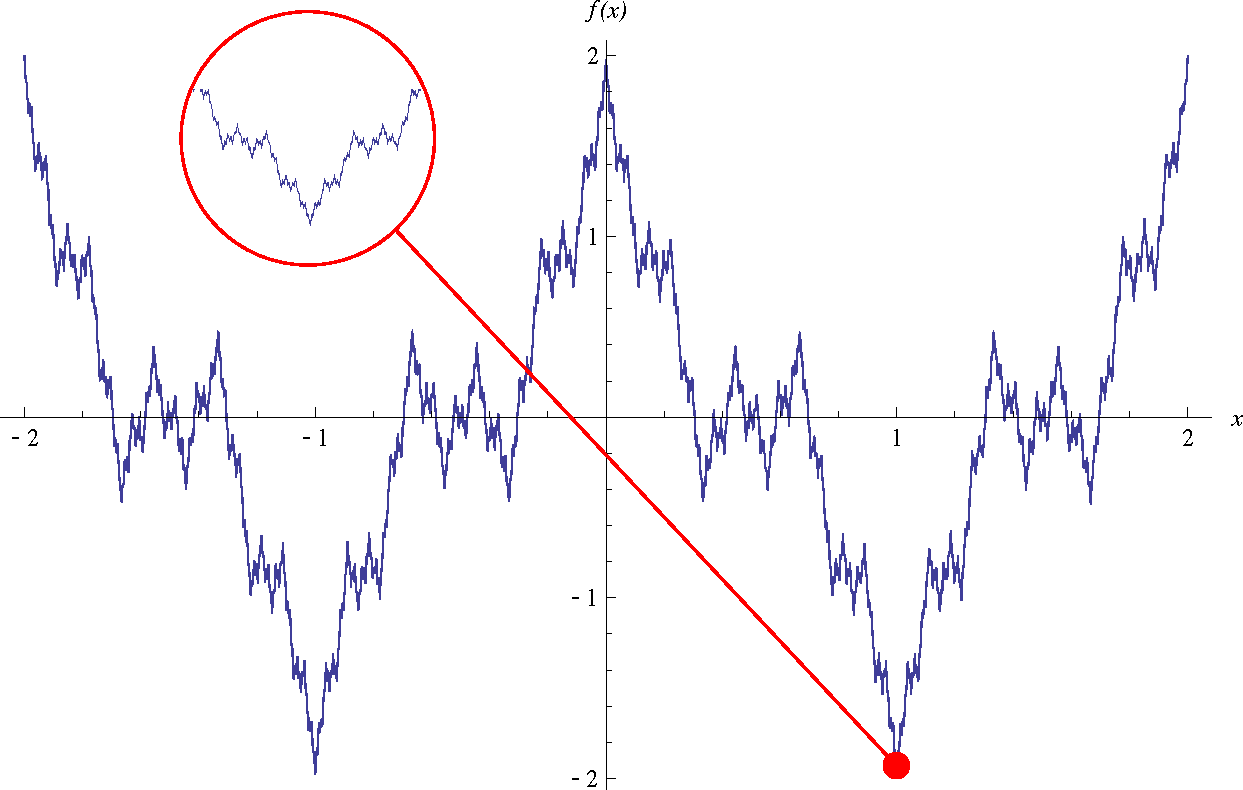
\includegraphics[width=10cm]{attachment/WeierstrassFunction.pdf}
	\caption{Weierstrass函数示意图, 图源Wikipedia}
\end{figure}

我们考虑证明$f$在任意一点不存在导数, 也就是让任意点处的斜率为无穷大. 固定$x$, 首先计算$$\frac{f(x+h)-f(x)}{h} = \sum_{n=0}^{\infty} a^n \frac{\cos (b^n\pi (x+h)) - \cos (b^n\pi x)}{h} = \sum_{n=0}^{m-1}(\cdots) + \sum_{n=m}^{\infty}(\cdots).$$
希望得到$$\left| \frac{f(x+h)-f(x)}{h} \right| \geq \left| \sum_{n=m}^{\infty}(\cdots) \right| - \left| \sum_{n=0}^{m-1}(\cdots) \right| > (\cdots ) \to +\infty .$$
因此需要估计(绝对值下)前一部分的上界和后一部分的下界. 先利用中值定理估计前一部分: 
\begin{align*}
	\left| \sum_{n=0}^{m-1}(\cdots) \right| &\leq \pi \sum_{n=0}^{m-1} (ab)^n \left| \frac{\cos (b^n\pi (x+h)) - \cos (b^n\pi x)}{b^n \pi h} \right| = \pi \sum_{n=0}^{m-1} (ab)^n |\sin (b^n\pi (x+\theta _n h))| \\ 
	&\leq \pi \sum_{n=0}^{m-1} (ab)^n = \pi \frac{(ab)^m-1}{ab-1}. 
\end{align*}
接下来, 令$b^mx=\alpha _m+\beta _m$, 其中$\alpha _m$是整数而$-1/2 \leq \beta _m < 1/2$. 于是$$\cos (b^n\pi x) = \cos (b^{n-m}\pi (\alpha _m + \beta _m)) = \cos (b^{n-m}\pi \alpha _m)\cos (b^{n-m}\pi \beta _m) = (-1)^{\alpha _m} \cos (b^{n-m}\pi \beta _m), $$
$$\cos (b^n\pi (x+h)) = \cos \left( b^{n-m}\pi(\alpha _m + \beta _m + b^mh) \right). $$
为了尽量化简, 可以令$b^mh=1-\beta _m$, 于是$\cos (b^n\pi (x+h)) = (-1)^{\alpha _m+1}$. 进而$$\left| \sum_{n=m}^{\infty}(\cdots) \right| = \frac{1}{|h|} \sum_{n=m}^{\infty} a^n(1+\cos (b^{n-m}\pi \beta _m)) > \frac{1}{h}a^m(1+\cos (\pi \beta _m)) > \frac{a^m}{h} > \frac{2}{3}(ab)^m. $$
其中关于$h$的放缩是因为$h = \frac{1-\beta _m}{b^m} \in [\frac{1}{2b^m},\frac{3}{2b^m}]$. 于是我们有$$\left| \frac{f(x+h)-f(x)}{h} \right| > (ab)^m \left( \frac{2}{3}-\frac{\pi}{ab-1} \right).$$
当$ab>1+\frac{3}{2}\pi$时右侧为正, 令$m \to \infty$(同时$h \to 0$)即得$f$在$x$处导数不存在. 


\circled{C}~~$\pi$的定义与三角函数的周期: 

在之前的补充习题中我们用幂级数定义了三角函数$$\cos z = \frac{e^{\ic z}+e^{-\ic z}}{2}= \sum_{k=0}^{\infty} \frac{(-1)^kx^{2k}}{(2k)!},\qquad \sin z = \frac{e^{\ic z} - e^{-\ic z}}{2\ic} = \sum_{k=0}^{\infty} \frac{(-1)^kx^{2k+1}}{(2k+1)!}, $$
并且顺带证明了三角函数的和角公式. 但是对三角函数至关重要的$\pi$值仍然没有定义. 现在用分析的方法定义$\pi$: 

首先, 通过求导容易证明$\sin x$在$(0,\delta)$上单调递增, $\cos x$在$(0,\delta)$上单调递减, 其中$\delta$是某个比较小的正数. 特别地, 由对称性, 易知$\cos x$在$x=0$处取得极大值$1$. 

接着我们要证明存在$\alpha >0$使得$\cos x$在$(0,\alpha)$上单调递减且$\cos \alpha =0$(同时$\sin \alpha =1$, 注意符号!), 另一方面存在$\beta >0$使得$\sin x$在$(\alpha ,\beta)$上单调递减且$\sin \beta =0$(同时$\cos \beta = -1$), 然后将$\beta$定义为$\pi$. 

\begin{proof}
	以第一条为例. 考虑使得$\cos x$在$(0,\alpha)$为正的最大的$\alpha$, 存在性由下方推理保证: 假设$\cos x$在$(0,+\infty)$均为正, 则$(\sin x)' = \cos x>0$, 即$\sin x$在$(0,+\infty)$单调递增, 从而存在极限$l>0$. 但是$(\cos x)' = -\sin x \searrow -l$, 这与$\cos x$有下界矛盾. 
	
	既然$\alpha \in \R$, 由$\cos x$的连续性可得$\cos \alpha=0$, 进而$\sin \alpha =1$(否则$\sin x$不会在$(0,\delta)$单调递增). 
\end{proof}

现在来考虑三角函数的周期. 令$S(x)=-\sin (x+\pi), C(x)=-\cos (x+\pi)$, 那么$S'(x) = -\cos (x+\pi) = C(x)$, $C'(x) = \sin (x+\pi) = -S(x)$, $S(0)=0, C(0)=1$. 令$f(x)=\begin{pmatrix}
	\sin x \\ \cos x
\end{pmatrix}$, $F(x) = \begin{pmatrix}
	S(x) \\ C(x)
\end{pmatrix}$. 我们不加证明地认为方程$$\begin{cases}
	f'(x)=Jf(x) \\ f(0)=I
\end{cases},\quad J=\begin{pmatrix}
		0 & 1 \\ -1 & 0
	\end{pmatrix}, I=\begin{pmatrix}
		0 \\ 1
	\end{pmatrix}$$存在唯一解(不能直接用$f(x),F(x)$相除再求导来证明), 于是$F(x) \equiv f(x)$. 这就是说$$-\sin (x+\pi) = \sin x,\qquad -\cos (x+\pi) = \cos x. $$
进而$\sin x$和$\cos x$的最小正周期都是$2\pi$. 

\subsection{l’Hôpital法则}

相信读者在高中已经熟悉了l’Hôpital法则的使用, 现在我们给出严格证明. 实际上, l’Hôpital法则包括$$x \to a^+, \quad x\to a^-, \quad x \to a, \quad x \to +\infty , \quad x \to - \infty , \quad x \to \infty$$
六种极限过程和$$f(x),g(x) \to 0,\qquad g(x) \to \infty$$
两种极限情况的各种组合情况. 我们只需要证明$x \to a^+$下两种极限情况, 立即可以推出剩下的情况. 

\begin{theorem}{$0/0$型l’Hôpital法则}
	设$f,g$在$(a,b)$上可导, 且对任意$x \in (a,b)$, $g'(x) \neq 0$. 若
	
	\begin{center}
		$\displaystyle \lim_{x \to a^+} f(x) = 0, \lim_{x \to a^+} g(x) = 0, $
	\end{center}
	
	\noindent
	且极限$\lim_{x \to a^+} \frac{f'(x)}{g'(x)}$存在, 则极限$\lim_{x \to a^+} \frac{f(x)}{g(x)}$也存在, 而且有
	
	\begin{center}
		$\displaystyle \lim_{x \to a^+} \frac{f(x)}{g(x)} = \lim_{x \to a^+} \frac{f'(x)}{g'(x)}. $
	\end{center}
\end{theorem}
\begin{proof}
	不妨令$f(a)=g(a)=0$, 从而$f,g$在$[a,b)$上连续. 对任意$x \in (a,b)$, 取$h \in (0,x-a)$, 由Cauchy中值定理可知存在$\theta \in (0,1)$使得$$\frac{f'(a+\theta h)}{g'(a+\theta h)} = \frac{f(x)-f(a)}{g(x)-g(a)} = \frac{f(x)}{g(x)}. $$
	在上式中令$x \to a^+$, 则$h \to 0^+$, 那么$$\lim_{x \to a^+} \frac{f'(x)}{g'(x)} = \lim_{h \to 0^+} \frac{f'(a+\theta h)}{g'(a+\theta h)} = \lim_{x \to a^+} \frac{f(x)}{g(x)}. $$
\end{proof}

\begin{theorem}{$\bigcdot/\infty$型l’Hôpital法则}
	设$f,g$在$(a,b)$上可导, 且对任意$x \in (a,b)$, $g'(x) \neq 0$. 若
	
	\begin{center}
		$\lim_{x \to a^+} g(x) = \infty, $
	\end{center}
	
	\noindent
	且极限$\lim_{x \to a^+} \frac{f'(x)}{g'(x)}$存在, 则极限$\lim_{x \to a^+} \frac{f(x)}{g(x)}$也存在, 而且有
	
	\begin{center}
		$\displaystyle \lim_{x \to a^+} \frac{f(x)}{g(x)} = \lim_{x \to a^+} \frac{f'(x)}{g'(x)}. $
	\end{center}
\end{theorem}
\begin{remark}
	尽管这里的适用范围是$\bigcdot/\infty$, 但是当$\bigcdot$有限时显然极限值为$0$, 因此$\infty/\infty$型才是常用的说法. 
\end{remark}
\begin{proof}
	只需证明$$\liminf_{x\to a^+} \frac{f'(x)}{g'(x)} \leq \liminf_{x\to a^+} \frac{f(x)}{g(x)} \leq \limsup_{x\to a^+} \frac{f(x)}{g(x)} \leq \limsup_{x\to a^+} \frac{f'(x)}{g'(x)}.$$
	
	以右侧为例. 记$s = \limsup_{x\to a^+} \frac{f'(x)}{g'(x)}$. 任取$s_1>s$, 存在$\delta$使得任意$x \in (a,a+\delta)$有$\frac{f'(x)}{g'(x)} <s_1$. 另外, 对任意$x \in (a,a+\delta)$, 由Cauchy中值定理可知, 存在$\xi \in (x,a+\delta)$使得$$\frac{f(x)-f(a+\delta)}{g(x)-g(a+\delta)} = \frac{f'(\xi)}{g'(\xi)} <s_1. $$
	这就是说$$\frac{f(x)}{g(x)} < s_1\left( 1-\frac{g(a+\delta)}{g(x)} \right) + \frac{f(a+\delta)}{g(x)} \to s_1,\quad x \to a^+.$$
	由$s_1$选取的任意性, $\lim_{x \to a^+} \frac{f(x)}{g(x)} \leq s$. 
\end{proof}
\begin{remark}
	该证明与之前Stolz定理的证明几乎相同. 
\end{remark}

\newpage
\section*{一些习题 ~~\small 对应原书5.2,5.3习题} \label{sec:ex6.1}

\subsection*{A: 中值定理的应用}

归纳地定义$f$在$x_0$处的$k$阶有限差: $$\Delta f(x_0;h_1) := f(x_0+h_1)-f(x_0), \qquad \Delta ^kf(x_0;h_1,\cdots ,h_k) := \Delta ^{k-1} (\Delta f(x;h_k)) (x_0;h_1,\cdots ,h_k). $$

\circled{A1}-1~~设$f \in C^{n-1}([a,b])$, 且在$(a,b)$上存在$n$阶导数. 设$x_0+h_1,\cdots ,x_0+h_1+\cdots +h_n$均包含于$[a,b]$, 那么存在包含这些点的最小闭区间内的点$\xi$使得$$\Delta ^n f(x_0;h_1,\cdots ,h_n) = f^{(n)}(\xi) h_1\cdots h_n. $$

\circled{A1}-2~~特别地, 记$\Delta ^nf(x_0;h^n) := \Delta ^nf(x_0;h,\cdots ,h)$. 若$f^{(n)}(x_0)$存在, 则$$f^{(n)}(x_0) = \lim_{h \to 0} \frac{\Delta ^n f(x_0;h^n)}{h^n}. $$

\circled{A1}-3~~函数$f(x)=\begin{cases}
	x^3\sin \frac{1}{x} & x\neq 0 \\ 0 & x = 0
\end{cases}$满足$\displaystyle \lim_{h\to 0} \frac{\Delta ^2 f(0;h^2)}{h^2}$存在但$f^{(2)}(0)$不存在. 
\vspace{1em}

设$f \in C^n((-1,1))$, $\sup_{x\in (-1,1)} |f(x)| \leq 1$. 记$m_k(I) = \inf_{x \in I} |f^{(k)}(x)|$. 
\vspace{1em}

\circled{A2}-1~~若将$I$依次分为区间$I_1,I_2,I_3$, 则$$m_k(I) \leq \frac{1}{|I_2|} (m_{k-1}(I_1) + m_{k-1}(I_3)). $$

\circled{A2}-2~~记$\lambda = |I|$, 则$$m_k(I) \leq \frac{2^{\frac{k(k+1)}{2}} k^k}{\lambda ^k}. $$

\circled{A2}-3~~存在只与$n$有关的$\alpha _n$, 使得若$|f'(0)| \geq \alpha _n$, 则$f^{(n)}(x)$在$(-1,1)$上有至少$n-1$个不同的零点. 








\newpage
\section{Taylor公式}

\subsection{带Peano余项的Taylor公式}

回顾无穷小增量公式$$f(x)=f(x_0)+f'(x_0)(x-x_0)+o(x-x_0),\quad x \to x_0.$$
现在我们希望将右侧的误差进一步缩小, 也即寻找常数$a_0,a_1,a_2$使得$$f(x) = a_0 + a_1(x-x_0) + a_2(x-x_0)^2 +o((x-x_0)^2),\quad x \to x_0. $$
由于$f$在$x_0$处连续, 可知$f(x_0)=a_0$. 进一步有$$\frac{f(x)-f(x_0)}{x-x_0} = a_1 + a_2(x-x_0) + o(x-x_0),\quad x \to x_0\quad \Leftrightarrow \quad f'(x_0)=a_1. $$
最后, 计算可得$$\frac{f(x)-f(x_0)-f'(x_0)(x-x_0)}{(x-x_0)^2} = a_2 + o(1), \quad x \to x_0 \quad \Leftrightarrow \quad a_2 = \frac{1}{2} \lim_{x \to x_0} \frac{f'(x)-f'(x_0)}{x-x_0} = \frac{1}{2}f''(x_0).$$
其中“$\Rightarrow$”方向使用了l’Hôpital法则, “$\Leftarrow$”方向是直接验证. 利用数学归纳法可以将这个想法推广: 

\begin{theorem}{带Peano余项的Taylor公式}
	设$f$在$x_0$附近有定义, 且在$x_0$处存在$n$阶导数. 则当$x \to x_0$时, $$f(x)=f(x_0)+\frac{1}{1!}f'(x_0)(x-x_0) + \cdots \frac{1}{n!}f^{(n)}(x_0)(x-x_0)^n + o((x-x_0)^n). $$
\end{theorem}
\begin{remark}
	最后的余项也可写作$O((x-x_0)^{n+1})$, 原因之前解释过. 
\end{remark}
\begin{remark}
	一般记$P_n(f,x_0;x)=f(x_0) + \cdots + \frac{1}{n!}f^{(n)}(x_0)(x-x_0)^n$为$f$在$x_0$处的$n$次Taylor多项式. 
\end{remark}
\begin{proof}
	归纳证明. 当$n=1$时显然. 假设当$n=k$时成立, 计算可得$$P'_{k+1}(f,x_0;x) = f'(x_0)+\frac{1}{1!}f''(x_0)(x-x_0) + \cdots + \frac{1}{k!}f^{(k+1)}(x_0)(x-x_0)^k = P_k(f',x_0;x).$$
	结合l’Hôpital法则, 我们有$$\lim_{x \to x_0} \frac{f(x)-P_{k+1}(f,x_0;x)}{(x-x_0)^{k+1}} = \frac{1}{k+1} \lim_{x \to x_0} \frac{f'(x)-P_k(f',x_0;x)}{(x-x_0)^k}=0.$$
	这就是说, $f(x)=P_{k+1}(f,x_0;x)+o((x-x_0)^{k+1})$. 
\end{proof}

为了让Taylor展开式尽可能简单, 我们习惯于令$x_0=0$, 得到的展开式称作\textit{Maclaurin展开式}. 现在来求一些函数的Maclaurin展开式(本质上就是求高阶导数): 

\begin{example}
	求$f(x)=\sin x$的Maclaurin展开式. 
\end{example}
\begin{solution}
	熟知$$\sin ^{(4k)} (x) = \sin x,\quad \sin ^{(4k+1)} (x) = \cos x,\quad \sin ^{(4k+2)} (x) = -\sin x,\quad \sin ^{(4k+3)} (x) = -\cos x. $$
	于是$f^{(2\ell )}(0)=0,f^{(2\ell +1)}(0)=(-1)^{\ell}$. 那么$$\sin x = x-\frac{1}{3!} x^3 + \cdots + \frac{(-1)^n}{(2n+1)!}x^{2n+1} + o(x^{2n+2}),\quad x\to 0.$$
\end{solution}

\begin{example}
	求$f(x)=\arctan x$的Maclaurin展开式. 
\end{example}
\begin{solution}
	由$f'(x)=(1+x^2)^{-1}$, 可知$(1+x^2)f'(x)=1$. 对两边求$k$阶导, 由Leibniz公式我们有$$(1+x^2)f^{(k+1)}(x) + 2kxf^{(k)}(x) + k(k-1)f^{(k-1)}(x)=0. $$
	令$x=0$, 即得递推关系$f^{(k+1)}(x)=-k(k-1)f^{k-1}(x)$. 于是$$\arctan x = x-\frac{1}{3}x^3+\cdots \frac{(-1)^n}{2n+1}x^{2n+1} + o(x^{2n+2}),\quad x\to 0. $$
\end{solution}

用类似的方法, 不难求得以下函数的Maclaurin展开式: 
\begin{itemize}
	\item $\displaystyle e^x = 1 + \frac{1}{1!}x + \cdots + \frac{1}{n!} x^n + o(x^{n}),\quad x\to 0.$
	\item $\displaystyle \ln (1+x) = x - \frac{1}{2}x^2 + \cdots + \frac{(-1)^{n-1}}{n} x^n + o(x^{n}),\quad x \to 0. $
	\item $\displaystyle (1+x)^{\alpha} = 1 + \frac{\alpha}{1!}x + \cdots \frac{\alpha \cdots (\alpha -n+1)}{n!} x^n + o(x^{n}),\quad x \to 0.$
	\item $\displaystyle \sin x = x-\frac{1}{3!} x^3 + \cdots + \frac{(-1)^n}{(2n+1)!}x^{2n+1} + o(x^{2n+2}),\quad x\to 0.$
	\item $\displaystyle \cos x = 1-\frac{1}{2!} x^2 + \cdots + \frac{(-1)^n}{(2n)!}x^{2n} + o(x^{2n+1}),\quad x\to 0.$
	\item $\displaystyle \arctan x = x-\frac{1}{3}x^3+\cdots \frac{(-1)^n}{2n+1}x^{2n+1} + o(x^{2n+2}),\quad x\to 0.$
	\item $\displaystyle \sinh x = x+\frac{1}{3!} x^3 + \cdots + \frac{1}{(2n+1)!}x^{2n+1} + o(x^{2n+2}),\quad x\to 0.$
	\item $\displaystyle \cosh x = 1+\frac{1}{2!} x^2 + \cdots + \frac{1}{(2n)!}x^{2n} + o(x^{2n+1}),\quad x\to 0.$
	\item $\displaystyle \artanh x = x+\frac{1}{3}x^3+\cdots \frac{1}{2n+1}x^{2n+1} + o(x^{2n+2}),\quad x\to 0. $
\end{itemize}

若要计算$\tan x$的Taylor展开, 我们需要Bernoulli数, 但这就是组合数学研究的对象了. 

另外, 我们观察到, 如$\sin x,\cos x,e^x$等函数的Maclaurin展开式和其幂级数形式非常类似(之后会介绍原因). 但是需要注意, 不能想当然地认为Maclaurin展开式直接可以推广为幂级数, 我们本质上还是在研究函数在一点处的性质. 反例如: 

\begin{example}
	设$f(x)=\begin{cases}
		e^{-\frac{1}{x^2}} & x \neq 0 \\ 0 & x = 0
	\end{cases}$. 则$f(x)=o(x^n)$对任意$n>0$成立. 
\end{example}
\begin{proof}
	计算可得$$f'(0)=\lim_{x \to 0} \frac{e^{-\frac{1}{x^2}}}{x} = 0,\quad f'(x)=\frac{2}{x^3}e^{-\frac{1}{x^2}},x \neq 0.$$
	通过猜测结合归纳法, 可以证明$$f^{(n)}(0) = 0,\quad f^{(n)}(x) = P_n(x)e^{-\frac{1}{x^2}},x \neq 0.$$
	其中$P_n(x)$满足如下递推关系: $P_0(x)=1,P_n(x)=\frac{2}{x^3}P_{n-1}(x)+P'_{n-1}(x)$. 
\end{proof}

这个例子同时能说明, 单纯提高Taylor多项式的次数不一定减小逼近误差. 

类似于微分最佳逼近定理, 我们有: 

\begin{theorem}{Taylor多项式最佳逼近定理}
	设$f$在$x_0$处存在$n$阶导数, 则对任意不等于$P_n(f,x_0;x)$且次数不超过$n$的多项式$P$, 均存在$\delta >0$使得对任意$x \in \mathring{N}_{\delta}(x_0)$都有$$|f(x)-P_n(f,x_0;x)| < |f(x)-P|.$$
\end{theorem}
\begin{proof}
	略. (提示: 对$P$应用Taylor展开)
\end{proof}

局部的Taylor公式通常用来求极限, 例如: 

\begin{example}
	求极限: $$\lim_{x\to 0} \frac{xe^x - \sin x -x^2}{\sin ^3 x}. $$
\end{example}
\begin{solution}
	首先将分母上的$\sin x$替换为$x$. 根据$\sin x = x - \frac{1}{3} x^3 + o(x^4)$和$e^x = 1+x+\frac{1}{2}x^2+o(x^3)$可知$$\textit{原式} = \lim_{x\to 0} \frac{1}{x^3}\left( x+x^2+\frac{1}{2}x^3 - x + \frac{1}{3}x^3 - x^2 +o(x^4) \right) = \frac{5}{6}. $$
\end{solution}


\subsection{对Taylor公式余项的定量研究}

之前介绍的带Peano余项的Taylor公式其实并没有真正给出余项$f(x)-P_n(f,x_0;x)$的值, 只是给出了余项的一个最终上界$(x-x_0)^{n+1}$. 类似于从无穷小增量公式到中值定理, 我们希望找到某个具体值$\xi$来描述余项. 

先从简单的情况写起: 设$f$具有待定的性质. $\varphi$在$[x_0,x]$上连续, 在$(x_0,x)$上可导且导数不为$0$. 首先由Cauchy中值定理, 存在$\xi \in (x_0,x)$使得
\begin{equation}
	\frac{f(x)-f(x_0)}{\varphi (x)-\varphi (x_0)} = \frac{f'(\xi)}{\varphi '(\xi)} \quad \Leftrightarrow \quad f(x) = P_0(f,x_0;x) + \frac{\varphi (x)-\varphi (x_0)}{\varphi '(\xi)} f'(\xi). \label{eq:taylor0}
\end{equation}

进一步, 我们希望右边仍然存在一个$P_1(f,x_0;x)$. 考虑令$F(t)=f(x)-(f(t)+f'(t)(x-t))$, 从而$F(x)-F(x_0)$恰好等于$f(x)-P_1(f,x_0;x)$. 现在, 对$F(t),\varphi (t)$应用Cauchy中值定理可知, 存在$\xi \in (x_0,x)$使得
\begin{equation}
	\frac{F(x)-F(x_0)}{\varphi (x)-\varphi (x_0)} = \frac{F'(\xi)}{\varphi '(\xi)} \quad \Leftrightarrow \quad f(x) = P_1(f,x_0;x) + \frac{\varphi (x) - \varphi (x_0)}{\varphi '(\xi)} f''(\xi)(x-\xi). \label{eq:taylor1}
\end{equation}

根据式\ref{eq:taylor0}和\ref{eq:taylor1}可以猜测下方定理的形式: 

\begin{theorem}{带定量余项的Taylor公式}
	设$f$在$(x_0,x)$上存在$n+1$阶导数, 在$[x_0,x]$上$n$-阶连续可导. 则对于在$[x_0,x]$上连续, 在$(x_0,x)$上可导且导数不为$0$的函数$\varphi$, 存在$\xi \in (x_0,x)$使得
	\begin{center}
		$\displaystyle f(x)=P_n(f,x_0;x) + \frac{\varphi (x) - \varphi (x_0)}{\varphi '(\xi) n!} f^{(n+1)}(\xi) (x-\xi )^n. $
	\end{center}
\end{theorem}
\begin{remark}
	将条件改为$(x,x_0)$和$[x,x_0]$也成立. 
\end{remark}
\begin{proof}
	构造函数$F(t)=f(x)-P_n(f,t;x)$. 显见$F$在$[x_0,x]$连续, 在$(x_0,x)$可导, 且$F'(t) = -\frac{f^{(n+1)}(t)}{n!}(x-t)^n$. 对$F(t),\varphi (t)$应用Cauchy中值定理, 则存在$\xi \in (x_0,x)$使得$$\frac{F(x)-F(x_0)}{\varphi (x)-\varphi (x_0)} = \frac{F'(\xi)}{\varphi '(\xi)}\quad \Leftrightarrow \quad \frac{P_n(f,x_0;x)}{\varphi (x)-\varphi (x_0)} = -\frac{f^{(n+1)}(\xi)}{\varphi '(\xi) n!}(x-\xi)^n. $$
\end{proof}

由这个定理, 马上可以得到两个常用推论: 

\begin{corollary}{带Lagrange余项的Taylor公式}
	设$f$在$(x_0,x)$上存在$n+1$阶导数, 在$[x_0,x]$上$n$-阶连续可导. 则存在$\xi \in (x_0,x)$使得
	\begin{center}
		$\displaystyle f(x)=P_n(f,x_0;x)+\frac{f^{(n+1)}(\xi)}{(n+1)!} (x-x_0)^{n+1}. $
	\end{center}
\end{corollary}
\begin{proof}
	令$\varphi (t) = (x-t)^{n+1}$即可. 
\end{proof}

\begin{corollary}{带Cauchy余项的Taylor公式}
	设$f$在$(x_0,x)$上存在$n+1$阶导数, 在$[x_0,x]$上$n$-阶连续可导. 则存在$\xi \in (x_0,x)$使得
	\begin{center}
		$\displaystyle f(x)=P_n(f,x_0;x)+\frac{f^{(n+1)}(\xi)}{n!} (x-\xi)^n(x-x_0). $
	\end{center}
\end{corollary}
\begin{proof}
	令$\varphi (t) = x-t$即可. 
\end{proof}

实际上, 令$\varphi (t) = (x-t)^p$可以得到更一般的结果, 称作\textit{带Schlömilch余项的Taylor公式}. 

可以利用带Lagrange/Cauchy余项的Taylor公式估计(在$0$处Taylor多项式的)误差. 我们注意到两种公式得到的误差分别为$$\frac{f^{(n+1)}(\theta x)}{(n+1)!} x^{n+1},\qquad \frac{f^{(n+1)}(\theta x)}{n!}(1-\theta)^n x^{n+1}.$$
其中$\theta \in (0,1)$. 

\subsection{Taylor级数}

\begin{theorem}{}
	设Taylor公式的余项$R_n(x):=f(x)-P_n(f,x_0;x)$. 若$R_n(x)$在$[a,b]$上逐点收敛到$0$, 则$f$在$[a,b]$上存在\textit{Taylor级数}展开式$$f(x) = \sum_{n=0}^{\infty} \frac{f^{(n)}(x_0)}{n!} (x-x_0)^n.$$
	特别地, 若$R_n(x)$一致收敛, 则Taylor级数也一致收敛. 
\end{theorem}
\begin{proof}
	显然. 
\end{proof}

\begin{example}
	证明以$e=\lim_{n\to \infty} (1+\frac{1}{n})^n$方式定义的指数函数$e^x$在$\R$上具有幂级数形式$$e^x = \sum_{n=0}^{\infty} \frac{x^n}{n!}. $$
\end{example}
\begin{proof}
	之前我们证明过$\lim_{x \to 0} \frac{e^x-1}{x}=1$, 进而得到了$(e^x)'=e^x$, 于是幂级数的部分和就是$P_n(e^x,0;x)$. 另一方面, 利用Lagrange余项, 当$|x|<M$时, 我们有$$|R_n(x)| = \left| \frac{e^{\theta x}}{(n+1)!} x^{n+1} \right| < \frac{e^M}{(n+1)!}M^{n+1} \to 0,\quad n \to \infty .$$
	因此对任意$M>0$, $e^x$在$[-M,M]$上具有上述幂级数形式. 令$M \to +\infty$即证. 
\end{proof}

\begin{example}
	证明以几何的方法定义出的正弦函数$\sin x$在任意有界闭区间上一致收敛于下列幂级数$$\sin x = \sum_{n=0}^{\infty} (-1)^n \frac{x^{2n+1}}{(2n+1)!}.$$
\end{example}
\begin{proof}
	同上, 利用Lagrange余项, 对于$|x|<M$, 只需证明$\sup_{x \in [-M,M]} |R_n(x)| \to 0$. 计算可得: $$\sup_{x \in [-M,M]} |R_{2n+1}(x)| = \sup_{x \in [-M,M]} \left| \frac{(-1)^{n+1}\sin \theta x}{(2n+2)!} x^{2n+2} \right| \leq \frac{M^{2n+2}}{(2n+2)!} \to 0.$$
\end{proof}

\begin{example}
	证明以$e=\lim_{n\to \infty} (1+\frac{1}{n})^n$方式定义的对数函数$\ln (1+x)$在$(-1,1]$上具有幂级数形式$$\ln (1+x) = \sum_{n=1}^{\infty} \frac{(-1)^{n+1}x^n}{n}. $$
\end{example}
\begin{proof}
	熟知$(\ln (1+x))^{(n)} = \frac{(-1)^{n-1}(n-1)!}{(1+x)^n}$, 从而Lagrange余项和Cauchy余项分别为$$R_n(x) = \frac{(-1)^n}{(1+\theta x)^{n+1}} \cdot \frac{(\theta x)^{n+1}}{n+1},\qquad R_n(x) = \frac{(-1)^n}{(1+\theta x)^{n+1}} (1-\theta)^nx^{n+1}. $$
	当$x \in (0,1]$时, 由Lagrange余项, $$|R_n(x)| = \frac{1}{n+1} \left( \frac{\tehta x}{1+\theta x} \right)^{n+1} \leq \frac{1}{n+1} \to 0.$$
	当$x \in (-1,1)$时, 由Cauchy余项, $$|R_n(x)| = \frac{|x|^{n+1}}{|1+\theta x|} \left( \frac{1-\theta }{1+\theta x} \right)^n \leq \frac{|x|^{n+1}}{1-|x|} \to 0.$$
\end{proof}

\begin{example}
	证明$(1+x)^{\alpha}$在$(-1,1)$上具有幂级数形式$$(1+x)^{\alpha} = \sum_{n=0}^{\infty} \frac{\alpha (\alpha -1) \cdots (\alpha -n+1)}{n!} x^n. $$
\end{example}
\begin{proof}
	熟知$((1+x)^{\alpha})^{(n)} = \alpha (\alpha -1) \cdots (\alpha -n+1)(1+x)^{\alpha -n}$. 利用Cauchy余项, 
	\begin{align*}
		|R_n(x)| &= \left| \frac{\alpha (\alpha -1) \cdots (\alpha -n)(1+\theta x)^{\alpha -n-1}}{n!} (1-\theta)^n x^{n+1} \right| \\
		&= \left| \alpha \left( \frac{\alpha}{1}-1 \right) \cdots \left( \frac{\alpha}{n}-1 \right) (1+\theta x^{n+1})^{\alpha -1} x^{n+1} \right| \cdot \left| \frac{1-\theta}{1+\theta x} \right|^n \\
		&\leq \left| \alpha \left( \frac{\alpha}{1}-1 \right) \cdots \left( \frac{\alpha}{n}-1 \right) (1+\theta x^{n+1})^{\alpha -1} x^{n+1} \right| = \alpha x (1+\theta x^{n+1})^{\alpha -1} \prod_{k=1}^{n} \left| \frac{\alpha}{k}-1  \right||x|
	\end{align*}
	注意到当$k$足够大时, $|\frac{\alpha}{k}-1||x|<|x|<1$, 因此令$n\to \infty$即得$R_n(x) \to 0$. 
\end{proof}


\newpage
\section*{一些习题 ~~\small 对应原书5.3习题} \label{sec:ex6.2}

\subsection*{A: 利用Taylor公式进行估计}

\circled{A1}~~求$a,b$使得$f(x) = \cos x - \dfrac{1+ax^2}{1+bx^2}$在$x \to 0$时是尽量高阶的无穷小量. 
\vspace{1em}

\circled{A2}~~求$\displaystyle \lim_{x \to \infty} x\left( \frac{1}{e} - \left( \frac{x}{x+1} \right)^x \right)$. 
\vspace{1em}

设$f$在$I$上存在二阶导函数, 记$M_0=\sup_{x \in I}|f(x)|,M_1=\sup_{x \in I}|f'(x)|,M_2=\sup_{x \in I}|f''(x)|$. 
\vspace{1em}

\circled{A3}-1~~若$I=[-a,a]$, 则$$|f'(x)| \leq \frac{M_0}{a} + \frac{x^2+a^2}{2a}M_2. $$

\circled{A3}-2~~对任意区间$I$, 有$$M_1 \leq \begin{cases}
	2\sqrt{M_0M_2} & \textit{若} |I| \geq 2\sqrt{\frac{M_0}{M_2}} \\ \sqrt{2M_0M_2} & \textit{若} I=\R
\end{cases}. $$
且其中的$2$与$\sqrt{2}$是最佳常数. 
\vspace{1em}

\circled{A3}-3~~若$f$在$I$上存在$p$阶导函数, 且$M_0$和$M_p = \sup_{x \in \R} |f^{(p)}(x)|$有限, 则对任意$k=1,\cdots ,p$, $$M_k := \sup_{x \in \R} |f^{(k)}(x)| \leq 2^{ \frac{k(p-k)}{2} } M_0^{ 1-\frac{k}{p} } M_p^{\frac{k}{p}}. $$

设$f$在区间$I$上存在$n$阶导数. 
\vspace{1em}

\circled{A4}-1~~若$f$在$I$上有$n+1$个零点, 则存在$\xi \in I$使得$f^{(n)}(\xi) = 0$. 
\vspace{1em}

设$I$中的点$x_1<\cdots <x_p$. 由代数的知识, 容易证明存在唯一的$n-1$次多项式$L(x)$满足$f(x_i)=L(x_i), i=1,\cdots ,p$, 称之为Lagrange插值多项式. 
\vspace{1em}

\circled{A4}-2~~对任意$x \in I$, 存在$\xi \in I$使得$$f(x)-L(x) = \frac{(x-x_1)\cdots (x-x_n)}{n!}f^{(n)}(\xi). $$

设$n_1,\cdots ,n_p \in \N$满足$n_1+\cdots +n_p=n$. 
\vspace{1em}

\circled{A4}-3~~若对任意$k=\leq n_i-1$有$f^{(k)}(x_i)=0, i=1,\cdots ,p$, 则存在$\xi \in [x_1,x_p]$使得$f^{(n-1)}(\xi) = 0$. 
\vspace{1em}

由代数的知识, 同样可得存在唯一的$n-1$次多项式$H(x)$满足$f^{(k)}(x_i)=H^{(k)}(x_i), i=1,\cdots ,p$, 称之为Hermite插值多项式. 
\vspace{1em}

\circled{A4}-4~~对任意$x \in I$, 存在包含$x$和$x_i,i=1,\cdots ,p$的最小闭区间内的点$\xi$使得$$f(x) - H(x) = \frac{(x-x_1)^{n_1} \cdots (x-x_p)^{n_p}}{n!} f^{(n)}(\xi). $$


\newpage
\section{用微分学方法研究函数}

\subsection{函数的单调性与极值}

在之前我们已经证明过函数的导数与其单调性的关系, 总结如下: 设$f$在$[a,b]$上连续, 在$(a,b)$上可导. 若$f'(x)>0$, 则$f$严格单调递增, 但反过来不一定成立, 只能得到$f'(x)\geq 0$(如$f(x)=x^3$); $f'(x) \geq 0$等价于$f$单调不减; $f'(x) \equiv 0$等价于$f(x) \equiv {\rm const}$. 

由Fermat引理, 我们知道函数在某点取得极值的必要条件, 现在通过研究该点左右的导数值得到充分条件: 

\begin{proposition}{}
	设$f$在$x_0$的一个邻域$N(x_0)$内有定义, 在$x_0$处连续, 在$\mathring{N}(x_0)$内可导, 若: 
	\begin{itemize}
		\item $(\forall x \in \mathring{N}^-(x_0), f'(x)<0) \wedge (\forall x \in \mathring{N}^+(x_0), f'(x)<0)$, 则$f$在$x_0$无极值. 
		\item $(\forall x \in \mathring{N}^-(x_0), f'(x)<0) \wedge (\forall x \in \mathring{N}^+(x_0), f'(x)>0)$, 则$f$在$x_0$有严格极小值. 
	\end{itemize}
\end{proposition}
\begin{remark}
	该命题并没有要求$f$在$x_0$处可导. 例如$f(x)=|x|$在$0$处取得极小值, 不能用Fermat引理判定, 但是可以用该命题判定. 
\end{remark}
\begin{proof}
	以第二个为例. 可知$f$在$\mathring{N}^-(x_0)$严格单调递减, 在$\mathring{N}^+(x_0)$严格单调递增. 又$f$在$x_0$处连续, 那么对任意$\{ x_n \} \subseteq \mathring{N}^-(x_0),\{ y_n \} \subseteq \mathring{N}^+(x_0)$, 若$x_n \nearrow x_0, y_n \searrow x_0$, 则$f(x_n) \searrow f(x_0), f(y_n) \nearrow f(x_0)$, 这就是说$f(x_0)$是严格极小值. 
\end{proof}

特别地, 若$f$还在$x_0$处可导, 则$f$在$x_0$处取得极值当且仅当$f'(x)$在$x_0$处改变符号. 

不过上方命题仍然不是充要条件: 

\begin{example}
	设函数$f(x) = \begin{cases}
		2x^2+x^2\sin \frac{1}{x} & x \neq 0 \\ 0 & x=0
	\end{cases}$, 则$f$在$0$处有极小值, 但是对任意$\delta >0$, $f|_{(-\delta,\delta)}$不是单调函数. 
\end{example}
\begin{proof}
	显然有$f(x) \geq x^2 \geq 0$, 且取得等号当且仅当$x=0$, 因此$f(0)$是最小值(特别地是局部极小值). 但是$f'(x) = 4x+2x\sin \frac{1}{x}-\cos \frac{1}{x}$在任意的$(-\delta,\delta)$上不保持符号不变. 
\end{proof}

可以用高阶导数来具体地判断驻点的情况. 

\begin{proposition}{}
	设$f$在$x_0$的一个邻域$N(x_0)$内有定义, 在$x_0$处存在$n$阶导数, 且$f'(x_0) = \cdots = f^{(n-1)}(x_0) = 0$, $f^{(n)}(x_0) \neq 0$. 当$n$为奇数时, $f$在$x_0$无极值; 当$n$为偶数时, $f$在$x_0$有极值, 特别地当$f^{(n)}(x_0)>0$时为严格极小值, $f^{(n)}(x_0)<0$时为严格极大值. 
\end{proposition}
\begin{proof}
	由局部Taylor公式, $$f(x)-f(x_0) = \frac{1}{n!} f^{(n)}(x_0)(x-x_0)^n+o((x-x_0)^n) = \left( \frac{1}{n!} f^{(n)}(x_0) + \alpha (x) \right)(x-x_0)^n. $$
	其中$\alpha (x) \to 0,x \to x_0$. 当$x$足够接近$x_0$时, $\frac{1}{n!} f^{(n)}(x_0) + \alpha (x)$的符号与$f^{(n)}(x_0)$相同. 因此, 当$n$为奇数时, $f(x)-f(x_0)$变号, 故不存在极值; 当$n$为偶数时, $f(x)-f(x_0)$与$f^{(n)}(x_0)$的符号相同. 
\end{proof}

\subsection{函数的凸性}

\begin{definition}{凸函数}
	设$f:E \to \R$, 其中$E$是区间. 称$f$在$E$上是\textit{凸的}(convex)(或称\textit{下凸的}), 如果对任意$x,y \in I$和$t \in [0,1]$, 有$$f(tx+(1-t)y) \leq tf(x)+(1-t)f(y). $$
	类似地, 称$f$在$E$上是\textit{凹的}(concave)(或称\textit{上凸的}), 如果上方的不等式反向. 
\end{definition}
\begin{remark}
	特别地, 若不等号为严格的, 称$f$是严格凸/凹的. 
\end{remark}

从几何的观点看, 凸函数图像上的任意两点的连线都在函数图像的上方. 

\begin{figure}[H]
	\centering
	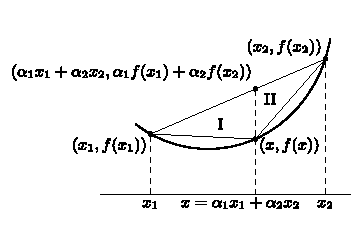
\includegraphics[width=8cm]{attachment/凸函数.pdf}
	\caption{凸函数示意图, 图源Zorich Fig. 5.11}
\end{figure}

凸函数的定义可以推广: 

\begin{theorem}{Jensen不等式}
	设$f:E \to \R$是凸函数, 其中$E$是区间. 则对任意$x_1,\cdots ,x_n \in E$和任意的$t_1,\cdots ,t_n \in [0,1]$, 如果$t_1+\cdots +t_n=1$, 则有
	\begin{center}
		$f(t_1x_1+\cdots +t_nx_n) \leq t_1f(x_1) + \cdots + t_nf(x_n). $
	\end{center}
\end{theorem}
\begin{proof}
	归纳即可. 
\end{proof}

\begin{proposition}{凸函数的等价条件}
	下列命题是等价的: 
	\begin{itemize}
		\item $f$在区间$E$上是凸函数. 
		\item 对于任意的$x,y,z \in E$, 若$x<y<z$, 则
		\begin{equation}
			\frac{f(y)-f(x)}{y-x} \leq \frac{f(z)-f(x)}{z-x} \leq \frac{f(z)-f(y)}{z-y}. \label{eq:凸函数等价定义}
		\end{equation}
		特别地, 若$f$是严格凸函数, 则上式中的不等号全部是严格的. 
		\item 集合$C=\{ (x,y):x\in E,y \geq f(x) \}$是凸集. 
	\end{itemize}
\end{proposition}
\begin{remark}
	若对任意$x,y \in C$和$t \in [0,1]$, $tx+(1-t)y \in C$, 则称$C$是凸集, 即是说$x,y$的连线仍在$C$中. 
\end{remark}
\begin{proof}
	(1) 若$f$是凸函数, 令$t=\frac{y-z}{x-z}$, 则$$f(y) = f(tx+(1-t)z) \leq tf(x)+(1-t)f(z) = \frac{y-z}{x-z}f(x) + \frac{x-y}{x-z}f(z).$$
	简单计算可知上式与式\ref{eq:凸函数等价定义}等价. 另一方面, 若式\ref{eq:凸函数等价定义}成立, 由$x,y,z$选取的任意性可知$f$是凸函数. 
\end{proof}

设$f$在$E$上可导. 我们注意到, 在式\ref{eq:凸函数等价定义}中令$y \to x$和$y \to z$, 有$$f'(x) \leq \frac{f(z)-f(x)}{z-x} \leq f'(z). $$
于是凸函数$f$的导数是单调不减的. 特别地, 若$f$是严格凸函数, 由Lagrange中值定理, 存在$x<\xi _1 < y < \xi _2 < z$使得$$f'(x) \leq f'(\xi _1) = \frac{f(y)-f(x)}{y-x} < \frac{f(z)-f(y)}{z-y} = f'(\xi _2) \leq f'(z).$$
于是$f$的导数是严格单调递增的. 

反过来, 用类似的方法可以证明, 若$f$的导数单调不减(严格单调递增), 则$f$是(严格)凸函数. 也就是说: 

\begin{proposition}{}
	设$E$是区间, $f:E \to \R$可导, 则$f$是(严格)凸函数当且仅当$f'$在$E$上单调不减(严格单调递增). 
\end{proposition}
\begin{remark}
	这个命题并不要求$f$存在二阶导数. 
\end{remark}

下面的命题说明, 就算没有$f$可导的假设, 凸性本身也可以诱导出分析的性质. 

\begin{proposition}{}
	设$E$是区间, $f:E \to \R$, 那么
	\begin{itemize}
		\item 对任意$x_0 \in \Int E$, $f$在$x_0$处的左右导数均存在(进而$f\in C(\Int E)$), 且$f'_-(x_0) \leq f'_+(x_0)$.
		\item 对任意$x,y \in \Int E$, 若$x<y$, 则
		\begin{center}
			$\displaystyle f'_-(x) \leq f'_+(x) \leq  \frac{f(y)-f(x)}{y-x} \leq f'_-(y) \leq f'_+(y).$
		\end{center}
	\end{itemize}
\end{proposition}
\begin{proof}
	(1) 由式\ref{eq:凸函数等价定义}可知对于$h_1,h_2>0$, $$\frac{f(x_0)-f(x_0-h_1)}{h_1} \leq \frac{f(x_0+h_2)-f(x_0)}{h_2}.$$
	特别地两侧分别关于$h_1,h_2$单调不减. 于是当$h_1 \to 0^-,h_2 \to 0^+$时, 两侧极限均存在, 且$f'_-(x_0) \leq f'_+(x_0)$. 
	
	(2) 同(1)可得$$\frac{f(x+h)-f(x)}{h} \leq \frac{f(y)-f(x)}{y-x}, $$
	在左侧令$h \to 0^+$, 即得$f'_+(x) \leq \frac{f(y)-f(x)}{y-x}$, 另一侧同理. 
\end{proof}

于是定义在闭区间上的凸函数只能在端点处不连续. 

另外, 既然$f$在每个点都存在左右导数, 我们可以研究左右切线: 

\begin{proposition}{}
	设$E$是区间, $f:E \to \R$是凸函数, $x_0 \in \Int E$, $\ell _k$表示过点$(x_0,f(x_0))$且斜率为$k$的直线. 则: 
	\begin{itemize}
		\item $f$的图像在$\ell _{f'_+(x_0)}$和$\ell _{f'_-(x_0)}$上方或重合. 
		\item $\ell _k$在$f$的图像之下或重合当且仅当$f'_-(x_0) \leq k \leq f'_+(x_0)$. 
	\end{itemize}
\end{proposition}
\begin{proof}
	(1) 以右极限情况为例, 只要证明对任意$x\neq x_0,x \in E$有$f(x) \geq f'_+(x_0)(x-x_0)+f(x_0)$, 当$x>x_0$时等价于$\frac{f(x)-f(x_0)}{x-x_0} \geq f'_+(x_0)$, 而这就是上方的命题. 当$x<x_0$时同理. 
	
	(2) 充分性显然. 必要性: 即当$x>x_0$时, $\frac{f(x)-f(x_0)}{x-x_0} \geq k$, 令$x \to x_0$即得$f'_+(x_0) \geq k$, 另一侧同理. 
\end{proof}

\begin{figure}[H]
	\centering
	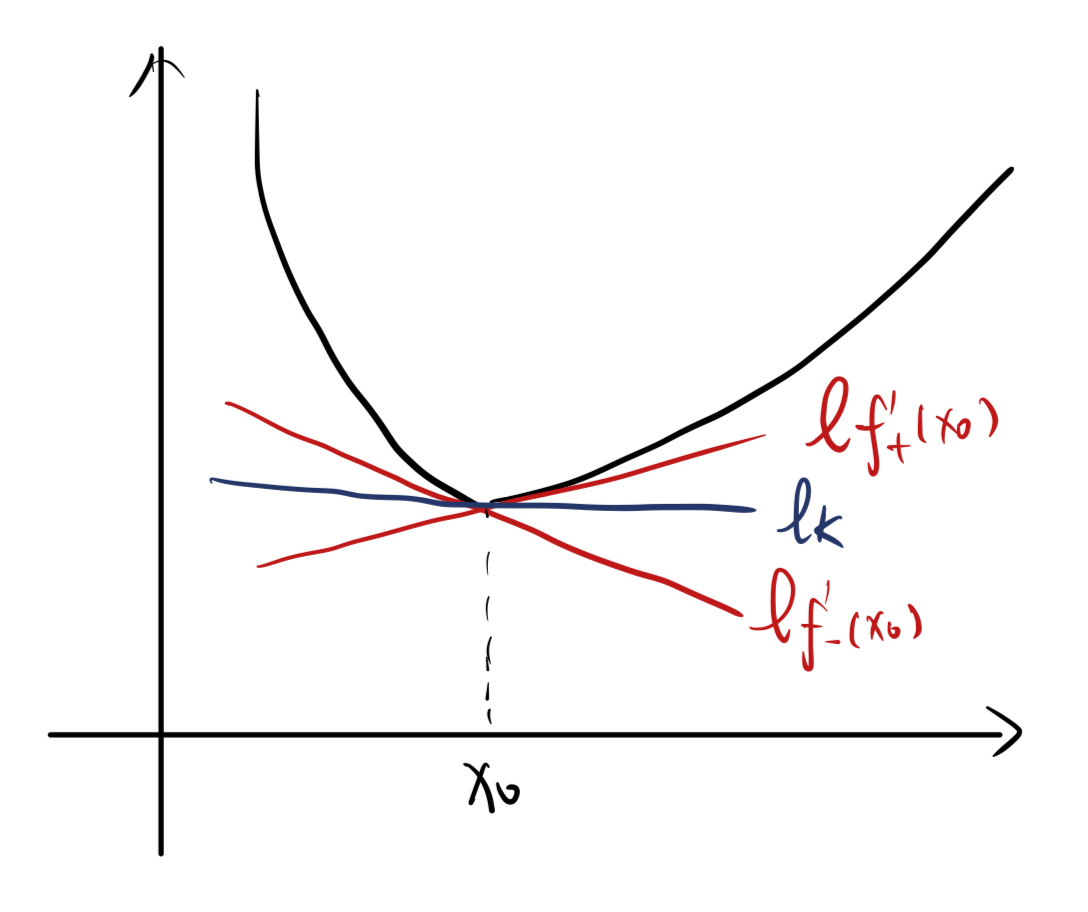
\includegraphics[width=6cm]{attachment/IMG_3552.jpg}
	\caption{凸函数的左右切线, 手绘勿喷}
\end{figure}

\newpage
\section{原函数与不定积分}

\begin{definition}{原函数}
	设$F$在区间$I$上可导. 称$F$为$f$在$I$上的一个\textit{原函数}(primitive function), 若$(F|_I)' = f|_I$. 
\end{definition}

由之前的命题, 不难证明$f(x)$在$I$上的所有原函数都是形如$F(x)+C$的形式. 于是可以定义:

\begin{definition}{不定积分}
	设$f$存在区间$I$上的原函数$F$, 则定义$f(x)$在$I$上的\textit{不定积分}(indefinite integration)为$$\int f(x) \dif x := \{ F(x)+C:C \in \R \}.$$
	亦可简写为$\int f(x) \dif x = F(x)+C$. 
\end{definition}

容易求得如下不定积分公式: 

\begin{figure}[H]
	\centering
	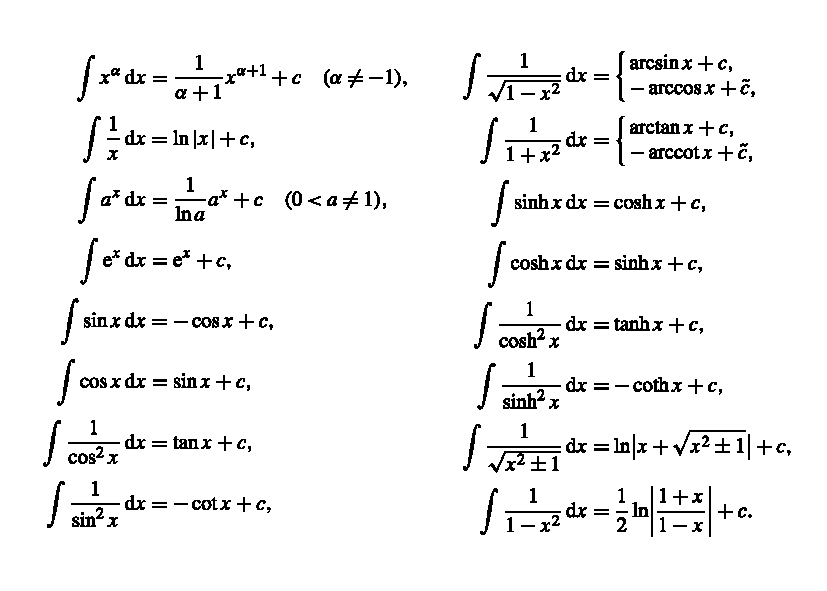
\includegraphics[width=14cm]{attachment/不定积分表.pdf}
	\caption{不定积分公式, 图源Zorich}
\end{figure}

利用微分的定义和性质, 还可以知道: 

\begin{proposition}{不定积分的简单性质}
	设$f$在区间$I$上的一个原函数$F$. 则: 
	\begin{itemize}
		\item $\displaystyle \dif \int f(x) \dif x = f(x) \dif x$. 
		\item $\displaystyle \int \dif F(x) = F(x) + C$. 
		\item $\displaystyle \int (\lambda f(x)+ \mu g(x)) \dif x = \lambda \int f(x) \dif x + \mu \int g(x) \dif x$. 
	\end{itemize}
\end{proposition}

下面介绍一些计算不定积分的公式和方法. 

\circled{A}~~换元积分法. 之前证明了$\dif v(u(x)) = v'(u(x)) \dif u(x)$. 在两侧同时求不定积分得$$\int \dif v(u(x)) = \int v'(u(x)) \dif u(x) \quad \Leftrightarrow \quad \int v'(u(x)) \dif u(x) = v(u(x)). $$

\begin{example}
	计算如下不定积分: $$1) \int \frac{x\dif x}{1+x^2};\qquad 2) \int \frac{\dif x}{\sin x}. $$
\end{example}
\begin{solution}
	(1) $$\int \frac{x\dif x}{1+x^2} = \frac{1}{2} \int \frac{\dif (1+x^2)}{1+x^2} = \frac{1}{2}\ln (1+x^2) +C.$$
	
	(2) $$\int \frac{\dif x}{\sin x} = \int \frac{\dif \frac{x}{2}}{\sin \frac{x}{2} \cos \frac{x}{2}} = \int \frac{\dif t}{\tan t \cos ^2 t} = \int \frac{\dif \tan t}{\tan t} = \ln \left| \tan \frac{x}{2} \right| + C.$$
\end{solution}

\circled{B}~~分部积分法: 之前证明了$\dif u(x)v(x) = (\dif u(x)) v(x) + u(x) (\dif v(x))$. 在两侧同时求不定积分得$$u(x)v(x) = \int v(x) \dif u(x) + \int u(x) \dif v(x). $$

\begin{example}
	计算如下不定积分: $$1) \int \ln x \dif x;\qquad 2) \int x^2e^x \dif x. $$
\end{example}
\begin{solution}
	(1) $$\int \ln x \dif x = x\ln x - \int e^{\ln x}\dif \ln x = x\ln x - x + C.$$
	
	(2) \begin{align*}
		\int x^2e^x \dif x &= \int x^2 \dif e^x = x^2e^x - \int e^x \dif x^2 = x^2e^x - 2\int xe^x \dif x \\
		&= x^2e^x - 2\int x \dif e^x = x^2e^x - 2\left( xe^x-\int e^x \dif x \right) = (x^2-2x+2)e^x + C. 
	\end{align*}
\end{solution}

\begin{example}
	计算如下不定积分: $$1) \int \cos (\ln x) \dif x;\qquad 2) \int \sin (\ln x) \dif x.$$
\end{example}
\begin{solution}
	计算可知$$\int \cos (\ln x) \dif x = \int x \dif \sin (\ln x) = x\sin (\ln x) - \int \sin (\ln x) \dif x,$$
	$$\int \sin (\ln x) \dif x = -\int x \dif \cos (\ln x) = -x\cos (\ln x) + \int \cos (\ln x) \dif x.$$
	于是$$\int \cos (\ln x) \dif x = \frac{1}{2}x(\sin (\ln x)+ \cos (\ln x)) +C,$$
	$$\int \sin (\ln x) \dif x = \frac{1}{2}x(\sin (\ln x)- \cos (\ln x)) +C.$$
\end{solution}

\circled{C}~~有理函数的不定积分. 我们熟知一个有理函数$\frac{P(x)}{Q(x)}$总是可以(在$\R$上)分解为一些形如$$\frac{1}{(x-a)^k},\qquad \frac{px+q}{(x^2+bx+c)^k}$$
的式子(其中$b^2<4c$)的线性组合. 于是只需要分别将两类式子的不定积分求出来: 
$$\int \frac{\dif x}{(x-a)^k} = \begin{cases}
	\frac{1}{-k+1}(x-a)^{-k+1}+C & k\neq 1 \\ \ln |x-a| + C & k=1
\end{cases}.$$
对于第二类, 令$u=x+\frac{b}{2}, a^2=c-\frac{b^2}{4}$, 于是$$\int \frac{px+q}{(x^2+bx+c)^k} \dif x = p \int \frac{u}{(u^2+a^2)^k} \dif u + \left(q-\frac{bp}{2} \right) \int \frac{\dif u}{(u^2+a^2)^k}.$$
其中$$\int \frac{u}{(u^2+a^2)^k} \dif u = \frac{1}{2} \int \frac{\dif (u^2+a^2)}{(u^2+a^2)^k} = \begin{cases}
	\frac{1}{2(1-k)}(u^2+a^2)^{1-k} & k\neq 1 \\ \frac{1}{2}\ln (u^2+a^2)
\end{cases}, $$
$$I_k = \int \frac{\dif u}{(u^2+a^2)^k} = \frac{u}{(u^2+a^2)^k} + 2k \int \frac{u^2}{(u^2+a^2)^{k+1}} \dif u = \frac{u}{(u^2+a^2)^k} + 2kI_k - 2ka^2I_{k+1}.$$
这样, 结合$$I_1 = \int \frac{\dif u}{u^2+a^2} = \frac{1}{a} \int \frac{\dif \frac{u}{a}}{1+(\frac{u}{a})^2} = \frac{1}{a} \arctan \frac{u}{a} + C,$$
我们就可以求出最终结果. 

\begin{example}
	计算如下不定积分: $$\int \frac{\dif x}{1+x^3}. $$
\end{example}
\begin{solution}
	注意到$1+x^3$的根为$-1,\frac{1+\sqrt{3}\ic}{2},\frac{1-\sqrt{3}\ic}{2}$, 于是不难求出$$\frac{1}{1+x^3} = \frac{\frac{1}{3}}{1+x} + \frac{-\frac{1}{3}x+\frac{2}{3}}{1-x+x^2}. $$
	现在开始计算: $$\int \frac{\dif x}{x+1} = \ln |x+1| + C,$$
	$$\int \frac{x-2}{x^2-x+1} \dif x = \int \frac{u-\frac{3}{2}}{u^2+\frac{3}{4}} \dif u = \frac{1}{2} \ln \left|u^2+\frac{3}{4} \right| -\sqrt{3} \arctan \left( \frac{2u}{\sqrt{3}} \right) + C.$$
	其中$u=x-\frac{1}{2}$. 所以$$\int \frac{\dif x}{1+x^3} = \frac{1}{3} \ln |x+1| - \frac{1}{6} \ln |x^2-x+1| + \frac{\sqrt{3}}{3}\arctan \left( \frac{2\sqrt{3}}{3}x-\frac{\sqrt{3}}{3} \right)+C.$$
\end{solution}

\circled{D}~~可有理化函数的不定积分. 

1. 设$R(u,v)=\frac{P(u,v)}{Q(u,v)}$. 为了将类似$R(\cos x,\sin x)$的式子变为关于$t$的有理函数, 我们可以利用如下换元: 
$$t=\tan \frac{x}{2},\qquad \int R(\cos x,\sin x) \dif x = \int R\left( \frac{1-t^2}{2t},\frac{2t}{1+t^2} \right) \frac{2\dif t}{1+t^2}, $$
$$t=\tan x,\qquad \int R(\cos ^2 x,\sin ^2 x) \dif x = \int R\left( \frac{1}{1+t^2},\frac{t^2}{1+t^2} \right) \frac{\dif t}{1+t^2}. $$
当然, 具体例题中常常使用其他三角变形公式和积分的换元公式来化简. 

\begin{example}
	计算如下不定积分: $$\int \frac{\dif x}{(\sin x + \cos x)^2}. $$
\end{example}
\begin{solution}
	\underline{\textbf{解法一}}~~令$t=\tan \frac{x}{2}$, 于是$$\int \frac{\dif x}{(\sin x + \cos x)^2} = \int \frac{\frac{2}{1+t^2}}{\left( \frac{2t}{1+t^2} + \frac{1-t^2}{1+t^2} \right)^2} \dif t = 2\int \frac{1+t^2}{(t^2-2t-1)^2} \dif t. $$
	之后利用有理函数的积分方法即可. 
	
	\underline{\textbf{解法二}}~~直接计算可得$$\int \frac{\dif x}{(\sin x + \cos x)^2} = \int \frac{\dif x}{\cos ^2x (1+\tan x)^2} = \int \frac{\dif \tan x}{(1+\tan x)^2} = -\frac{1}{1+\tan x}+C.$$
\end{solution}

2. 同上定义$R(u,v)$. 我们可做如下第二类化简: $$R\left( x,\sqrt[n]{\frac{ax+b}{cx+d}} \right) = R\left( \frac{dt^n-b}{-ct^n+a},t \right). $$
具体计算过于麻烦, 这里就不举例了. 

3. 同上定义$R(u,v)$. 考虑$R(x,\sqrt{ax^2+bx+c})$的情况. 实际上通过配方, 只需考虑如下三种简单形式: $$\int R(t,\sqrt{t^2+1}) \dif t, \qquad \int R(t,\sqrt{t^2-1}) \dif t, \qquad \int R(t,\sqrt{1-t^2}) \dif t. $$
Euler提出了针对这三种形式的代换: $$\sqrt{t^2+1}=tu\pm 1,t-u;\qquad \sqrt{t^2-1}=u(t\pm 1),t-u;\qquad \sqrt{1-t^2}=u(1\pm t),tu\pm 1. $$
右侧的式子都是可以取其相反数的. 当然另一种思路是利用三角/双曲换元. 
\begin{remark}
	考虑$R(x,\sqrt{P(x)})$的原函数, 其中$P(x)$是次数$n>2$的多项式. Abel和Liouville证明了这样的不定积分一般不能表示为初等函数. 我们称该积分在$n=3,4$时为\textit{椭圆积分}, 在$n>4$时为\textit{超椭圆积分}. 
\end{remark}

\begin{example}
	计算如下不定积分: $$\int \frac{\dif x}{x+\sqrt{x^2+2x+2}}. $$
\end{example}
\begin{solution}
	化简可得$$\int \frac{\dif x}{x+\sqrt{x^2+2x+2}} = \int \frac{\dif t}{t-1+\sqrt{t^2+1}}. $$
	其中$t=x+1$. 令$\sqrt{t^2+1}=u-t$, 于是$t=\frac{u^2-1}{2u}$, 进而$$\textit{原式} = \frac{1}{2} \int \frac{1+\frac{1}{u^2}}{u-1} \dif u = \int \frac{\dif u}{u-1} - \frac{1}{2} \int \frac{\dif u}{u^2} - \frac{1}{2} \int \frac{\dif u}{u} = \ln |u-1| - \frac{1}{2}\ln |u| + \frac{1}{2u} +C.$$
	其中$u=x+1+\sqrt{x^2+2x+2}$. 
\end{solution}






